\pagebreak
\thispagestyle{empty}
\movetoevenpage
\begin{figure}
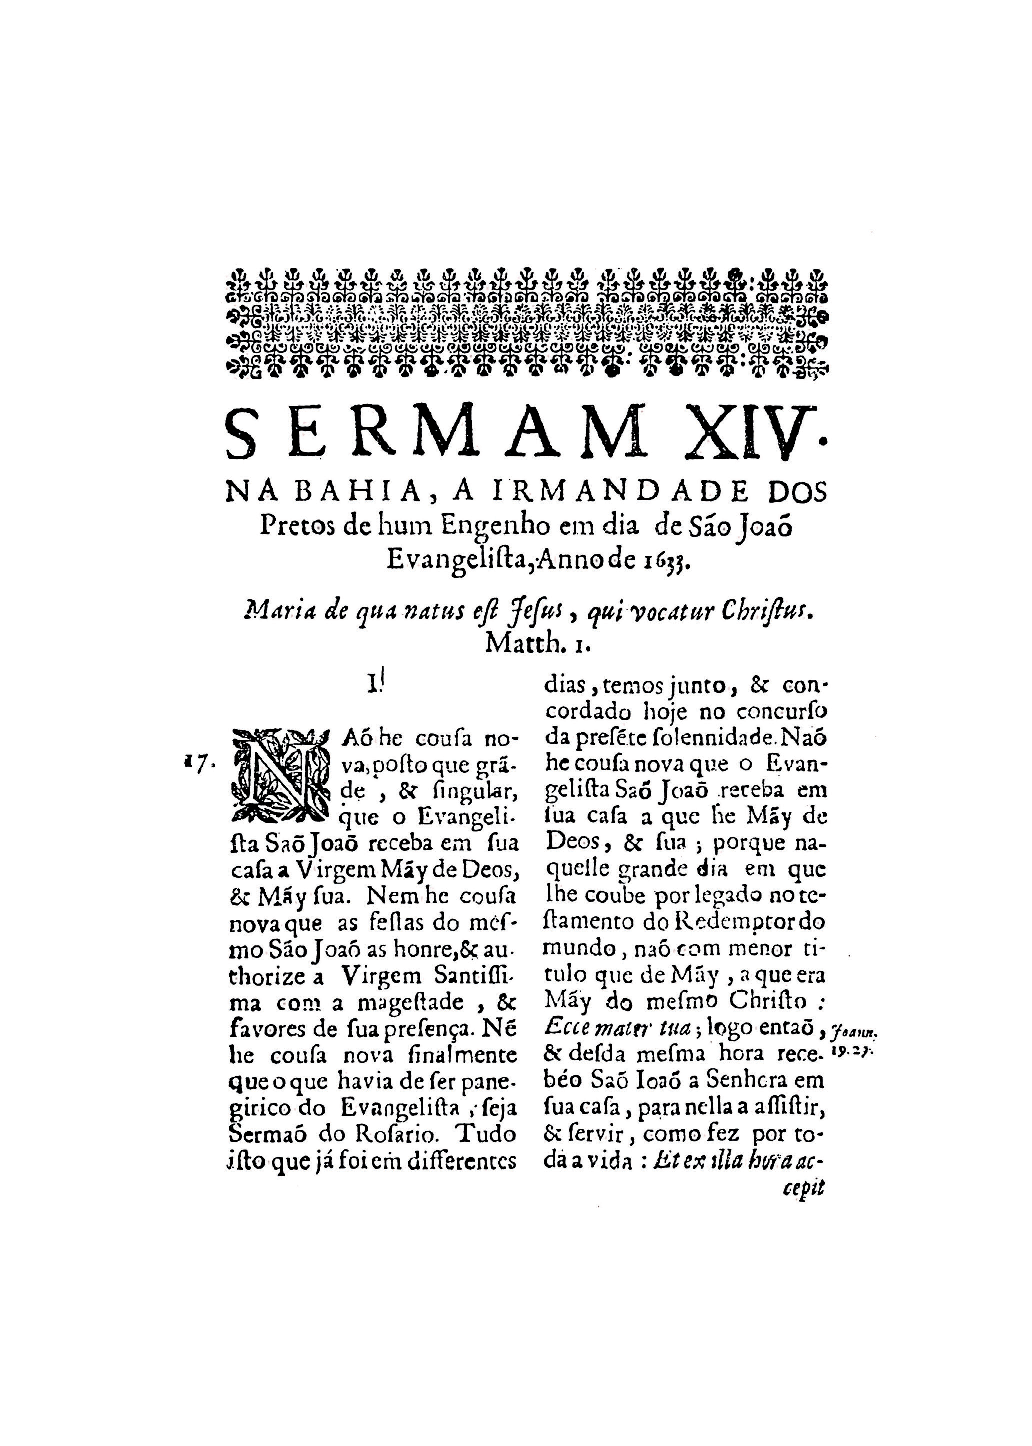
\includegraphics[width=\textwidth]{./imgs/rosa.pdf}  
\end{figure}

\chapter{Sermão \textsc{xiv} do Rosário}

\begin{quotation}
\noindent{}Na Bahia, à irmandade dos pretos de um Engenho
em dia de S.\,João Evangelista, Ano de 1633.
\end{quotation}

\epigraph{\emph{Maria de qua natus est Jesus, qui vocatur Christus}.\footnotemark}{Mt, 1.}\footnotetext{Mt 1[:16] [e Jacó gerou a José, marido de \textit{Maria, da qual nasceu Jesus, que se chama o Cristo}.]}

\section*{I}

\noindent{}Não é coisa nova, posto que grande e singular, que o
Evangelista S.\,João receba em sua casa a Virgem Mãe de Deus, e Mãe sua.
Nem é coisa nova que as festas do mesmo S.\,João as honre e autorize a
Virgem Santíssima com a majestade e favores de sua presença. Nem é coisa
nova, finalmente, que o que havia de ser panegírico do Evangelista, seja
Sermão do Rosário. Tudo isto que já foi em diferentes dias, temos junto
e concordado hoje no concurso da presente solenidade. Não é coisa nova
que o Evangelista S.\,João receba em sua casa a que é Mãe de Deus e sua;
porque naquele grande dia em que lhe coube por legado no testamento do
Redentor do mundo, não com menor título que de Mãe, a que era Mãe do
mesmo Cristo:~\emph{Ecce Mater tua};\footnote{Jo 19:27 [Depois, disse ao discípulo: \textit{Eis aí tua mãe. Edesde aquela hora o discípulo a recebeu em sua casa}.]} logo então e desde
a mesma hora recebeu S.\,João a Senhora em sua casa, para nela assistir e
servir, como fez por toda a vida:~\emph{Et ex illa hora accepit eam
Discipulus in sua}. E isto é o que torna a fazer hoje o
mesmo evangelista; porque chamando"-se em frase dos sagrados ritos casa
própria de cada um dos Santos aquele dia que a Igreja dedicou à sua
celebridade; neste dia e nesta casa recebe hoje S.\,João a Senhora,
dando"-lhe nela o lugar devido, que é o primeiro e principal. Nem é coisa
nova que as festas de S.\,João as honre e autorize a Virgem Santíssima
com a majestade e favores de sua presença; porque nas bodas de Caná de
Galileia o ser S.\,João o Esposo, foi a razão de se achar ali a
Senhora:~\emph{Et erat Mater Jesu ibi}.\footnote{Jo 2:1 [E, ao terceiro dia, fizeram-se umas bodas em Caná da Galiléia; \textit{e estava ali a mãe de Jesus}.]} E se foi favor
da sua piedade e assistência a conversão de água em vinho, não foi menor
graça, ou milagre da Virgem das Virgens, que S.\,João, por imitar sua
virginal pureza, renunciasse então o matrimônio, e o convertesse em
celibato. Finalmente, não é coisa nova, que o que havia de ser
panegírico do Evangelista, seja Sermão do Rosário, porque como se refere
nas Histórias Dominicanas, indo o Patriarca S.\,Domingos para pregar de
S.\,João em tal dia como hoje, ao tempo que recolhido a uma capela da
mesma Igreja se estava encomendando a Deus, lhe apareceu a Virgem Maria,
e lhe mandou que deixasse o Sermão que tinha meditado de S.\,João, e
pregasse o seu Rosário. Fê"-lo assim o grande Patriarca dos Pregadores, e
o fruto do Sermão que pelo zelo e eficácia do Pregador sempre costumava
ser grande, pela graça e virtude de quem o mandou pregar, foi naquela
ocasião muito maior, e mais patente com igual proveito e admiração dos
ouvintes.


Mas que fará cercado das mesmas obrigações, tantas e tão
grandes, quem não só falto de semelhante espírito, mas novo, ou noviço,
no exercício e na arte, é esta a primeira vez que subido indignamente a
tão sagrado lugar, há de falar dele em público?\footnote{Foi o primeiro Sermão que o Autor pregou em público antes de ser Sacerdote.} Vós,
soberana Rainha dos Anjos e dos homens, e Mãe da Sabedoria incriada (a
quem humildemente dedico as primícias daquelas ignorâncias que ainda se
não podem chamar estudos, como única Protetora deles) pois o dia e
assunto é, Senhora, de vossos maiores mistérios, vos dignais de me
assistir com a luz ou sombra da graça com que a virtude do Altíssimo no
primeiro de todos vos fez fecunda:~\emph{Ave Maria}.


\section*{II}

Temos hoje (por outro modo do que já o disse) três dias em
um dia, e três festas em uma festa: o dia e a festa de S.\,João, o dia e
festa da Senhora do Rosário, e o dia e a festa dos Pretos seus devotos.
E quando fora necessário termos também três Evangelhos; um só Evangelho
que nos propõe a Igreja, qual é? Posto que largo em nomes e gerações, é
tão breve e resumido no que finalmente vem a dizer, que todo se encerra
na cláusula que tomei por tema:~\emph{Maria de qua natus est Jesus, qui
vocatur Christus}. Se o Sermão houvera de ser do Nascimento de Cristo,
que é a solenidade do oitavário corrente, não podia haver outro texto,
nem mais próprio do tempo, nem mais acomodado ao Mistério: mas havendo
de pregar, não sobre este, senão sobre outros assuntos, e esses
não"-livres, senão forçados; e sendo os mesmos assuntos não menos que
três, e todos três tão diversos, como os poderei eu fundar sobre a
estreiteza de umas palavras, que só nos dizem que Jesus nasceu de
Maria:~\emph{Maria de qua natus est Jesus}? Suposto pois que nem é
lícito ao Pregador (se quer ser Pregador) apartar"-se do tema, nem o tema
nos oferece outra coisa mais que um Filho nascido de Maria;
multiplicando este nascimento em três nascimentos, este nascido em três
nascidos, e este Filho em três filhos, todos três nascidos de Maria
Santíssima; esta mesma será a matéria do Sermão, dividido também em três
partes. Na primeira veremos com novo nascimento nascido de Maria a
Jesus; na segunda com outro novo nascimento nascido de Maria a S.\,João;
e na terceira, também com novo nascimento nascidos de Maria aos Pretos
seus devotos. Deem"-me eles principalmente a atenção que devem, e destes
três nascimentos nascerão outros tantos motivos, com que reconheçam a
obrigação que têm de amar, venerar, e servir a Virgem Senhora Nossa,
como Mãe de Jesus, como Mãe de S.\,João, e como Mãe sua.

\section*{III}

Primeiramente digo que temos hoje nascido de Maria a Cristo
Senhor nosso, não como nasceu há três dias, mas com outro nascimento
novo. E que novo nascimento é este? É o nascimento com que nasceu da
mesma Mãe daqui a trinta e três anos, não em Belém, senão em Jerusalém.
Isto é o que diz o nosso texto: e provo:~\emph{Maria de qua natus est
Jesus, qui vocatur Christus}. Maria da qual nasceu Jesus, que se chama
Cristo. Cristo quer dizer ungido, Jesus quer dizer Salvador. E quando
foi Cristo Salvador, e quando foi ungido? Foi ungido na Encarnação, e
foi Salvador na Cruz. Foi ungido na Encarnação, quando unindo Deus a si
a Humanidade de Cristo, a exaltou sobre todas as criaturas, como diz
Davi:~\emph{Unxit te Deus, Deus tuus oleo laetitiae prae consortibus
tuis}.\footnote{Sl 44:8 [Tu amas a justiça e aborreces a impiedade; \textit{por isso, Deus, o teu Deus, te ungiu com óleo de alegria, mais do que a teus companheiros.}]} E foi Salvador na Cruz, quando por meio da
morte, e pelo preço de seu Sangue salvou o gênero humano, como diz S.\,Paulo:~\emph{Factus obediens usque; ad mortem, mortem autem crucis:
propter quod et Deus exaltavit illum, et donavit illi nomen, quod est
super omne nomen, ut in nomine Jesu omne
genuflectatur}.\footnote{Fl 2:8 [8-10] [e, achado na forma de homem, humilhou-se a si mesmo, sendo obediente até à morte e morte de cruz. \textit{Pelo que} também \textit{Deus o exaltou} soberanamente \textit{e lhe deu um nome que é sobre todo o nome, para que ao nome de Jesus se dobre todo joelho dos que estão nos céus, e na terra, e debaixo da terra}.]} Logo quando Cristo Senhor nosso nasceu
em Belém, propriamente nasceu Cristo, mas não nasceu Jesus, nem
Salvador: nasceu Cristo porque já estava ungido pela união Hipostática,
com que a Pessoa do Verbo se uniu à Humanidade: e não nasceu Jesus, nem
Salvador, porque ainda não tinha remido o mundo, nem o havia de remir e
salvar senão em Jerusalém daí a trinta e três anos.


Fala o profeta Isaías do parto virginal de Maria Santíssima
(como notaram S.\,Gregório Nisseno, e S.\,João Damasceno) e diz
assim:~\emph{Antequam parturiret, peperit: antequam veniret partus ejus,
peperit masculum}.\footnote{Is 66:7 [\textit{Antes que estivesse de parto, ela deu à luz; antes que lhe viessem as dores, ela deu à luz um filho}.]} Na primeira cláusula diz que pariu a
Senhora antes das dores do parto; que isso quer dizer:~\emph{Antequam
parturiret}: e na segunda diz que pariu antes do parto:~\emph{Antequam
veniret partus ejus, peperit}: Não é necessário que nós dificultemos o
passo, porque o mesmo Profeta confessa que disse uma coisa inaudita, e
que nunca se viu semelhante:~\emph{Qui audivit unquam tale, et quis
vidit huic simile?}\footnote{Is 66:8 [\textit{Quem jamais ouviu tal coisa? Quem viu coisas semelhantes?} Poder-se-ia fazer nascer uma terra em um só dia? Nasceria uma nação de uma só vez? Mas Sião esteve de parto e já deu à luz seus filhos.]} Que a bendita entre todas as
mulheres saísse à luz com o fruto bendito de seu ventre sem padecer
dores, privilégio era devido à pureza virginal, com que o concebeu, e
assim o confessa a nossa Fé. Mas que parisse antes do
parto:~\emph{Antequam veniret partus ejus}: como se pode entender, senão
supondo na mesma Senhora dois partos do mesmo Filho, e supondo também
que o primeiro parto foi sem dores, e o segundo com dores? Assim foi, e
assim o diz: quem? O nosso português Santo Antônio, que é bem preceda
agora a todos os outros Doutores da Igreja, pois falamos na
sua:~\emph{Beatae Mariae duplex fuit partus, unus in carne, alius in
spiritu. Partus carnis fuit virgineus, et omni gaudio plenus, quia
peperit sine dolore gaudium Angelorum. Secundus partus fuit dolorosus,
et omni amaritudine plenus, in Filii ejus passione, cujus animam
pertransivit gladius}. Sabeis por que faz menção Isaías de dois partos
da Virgem Beatíssima, e no primeiro nega as dores, e no segundo não? A
razão é (diz o Mestre Seráfico) porque este foi o modo e a diferença com
que a Senhora pariu a seu bendito Filho não uma, senão duas vezes: a
primeira vez sem dores, antes com júbilos de alegria, quando entre
cantares de Anjos o pariu no Presépio: a segunda vez com dores, e cheia
de amarguras, quando trespassada da espada de Simeão o tornou a parir ao
pé da Cruz. Uma vez nascido Cristo em Belém, e outra vez nascido em
Jerusalém: uma vez nascido no princípio da vida, e outra vez nascido no
fim dela: uma vez trinta e três anos antes, outra vez trinta e três anos
depois: que por isso o Profeta, falando deste segundo parto, disse
advertidamente:~\emph{Antequam veniret partus ejus}: porque um parto
depois do outro havia de tardar em vir tantos anos.

E posto que bastava por prova da minha proposta a autoridade
de tão grande intérprete das Escrituras como Santo Antônio, a quem por
essa causa chamaram os Oráculos de Roma Arca do Testamento; diga"-nos o
mesmo o evangelista S.\,João com texto mais claro que o de Isaías. No
Capítulo doze do seu Apocalipse viu S.\,João aquela mulher tão prodigiosa
como sabida, a quem vestia o Sol, calçava a Lua, e coroavam as Estrelas:
e diz que chegada a hora do parto, foram não só grandes, mas terríveis
as dores com que pariu um Filho varão, o qual havia de ser Senhor do
Mundo, e Governador de todas as gentes:~\emph{Cruciabatur ut pariat, et
peperit filium masculum, quirecturus erat omnes
gentes}.\footnote{Ap 12:2-5 [E estava grávida e com dores de parto e \textit{gritava com ânsias de dar à luz}.]; Ap 12:5 [\textit{E deu à luz um filho, um varão que há de reger todas as nações} com vara de ferro; e o seu filho foi arrebatado para Deus e para o seu trono.]} Esta mulher prodigiosa, em cujo ornato se
empenharam e despenderam todas as luzes do Céu, era a Virgem Santíssima:
o Filho Senhor do mundo, e que havia de governar todas as gentes, era
Cristo Governador do Universo, e Senhor dele. Mas se o parto da mesma
Virgem foi isento de toda a dor e moléstia, que dores e que tormentos
são estes com que agora S.\,João a viu parir, não outro, senão o mesmo
Filho? A palavra~\emph{Cruciabatur}, que é derivada da Cruz, basta por
comento de todo o texto. O Filho era o mesmo, e a Mãe a mesma, mas o
parto da Mãe, e o nascimento do Filho não era o mesmo, senão muito
diverso. Era o segundo nascimento do Filho, em que por modo superior a
toda a natureza havia de nascer morrendo. E porque este segundo
nascimento foi entre dores, tormentos, e afrontas, e com os braços
pregados nos de uma Cruz, por isso a mesma Cruz do nascimento do Filho
foi também a Cruz do parto da Mãe:~\emph{Et cruciabatur ut pariat}.


Nasceu o Filho crucificado na sua Cruz, e pariu"-o a Mãe
crucificada na Cruz do Filho: e se perguntarmos (que é o que só nos
resta) por que o Filho no segundo nascimento nasceu assim, e a Mãe o
pariu do mesmo modo? A razão, como dizia ao princípio, não foi outra
senão porque Cristo no primeiro parto nasceu propriamente Cristo, e
neste segundo nasceu propriamente Jesus. Esta foi a diferença com que o
Anjo anteontem anunciou aos Pastores o nascimento do mesmo
Cristo:~\emph{Quia natus est vobis hodie Salvator, qui est
Christus}:\footnote{Lc 2:11 [\textit{pois}, na cidade de Davi, \textit{vos nasceu hoje o Salvador, que é Cristo}, o Senhor.]} Alegrai"-vos, porque hoje nasceu o Salvador,
que é Cristo. Notai que não disse:~\emph{Qui est Salvator}, assim como
disse:~\emph{Qui est Christus}: porque o menino nascido já era Cristo,
mas ainda não era Salvador. Havia de ser Salvador, e para ser Salvador,
nascia, mas ainda o não era. Cristo sim,~\emph{Qui est Christus}; porque
já estava ungido na dignidade de Filho de Deus, mas na de Jesus, e de
Salvador ainda não; porque essa não a havia de receber no Presépio,
senão na Cruz:~\emph{Factus obediens usque; ad mortem crucis, ut in
nomine Jesu omne genuflectatur}. E aqui o que propriamente nasceu Jesus,
e não de outra Mãe, senão da mesma Virgem Maria:~\emph{Maria de qua
natus est Jesus}.


\section*{IV}

O segundo filho da mesma Virgem Maria, e nascido também no
Calvário, e com novo e segundo nascimento, foi São João. E que seria se
disséssemos que também deste nascimento se verifica o nosso texto? O em
que agora reparo nas palavras~\emph{de qua natus est Jesus, qui vocatur
Christus}, é que este~\emph{vocatur}~parece impróprio, e
este~\emph{Christus}~supérfluo. O nome próprio do Filho de Deus, e Filho
de Maria, é Jesus: este nome lhe foi posto no dia da Circuncisão, e
assim o tinha revelado o Anjo antes de ser concebido:~\emph{Vocatum est
nomen ejus Jesus, quod vocatum est ab Angelo priusquam in utero
conciperetur}.\footnote{Lc 2:21 [E, quando os oito dias foram cumpridos para circuncidar o menino, \textit{foi-lhe dado o nome de Jesus, que pelo anjo lhe fora posto antes de ser concebido}.]} Logo o~\emph{vocatur}~aplicado não ao
nome Jesus senão ao sobrenome~\emph{Christus}, parece impróprio: e o
mesmo sobrenome~\emph{Christus}~também parece supérfluo, porque só seria
necessário para distinguir um Jesus de outro Jesus. Porventura há outro
Jesus, e nascido de Maria, que se não chame Cristo? Digo que sim. Há um
Jesus Filho de Maria, que se chama Cristo; e há outro Jesus também Filho
de Maria, que se chama João. E por isso o Evangelista para distinguir um
Jesus de outro Jesus, e um Filho de Maria de outro Filho de Maria, não
supérflua, senão necessariamente acrescentou ao nome o sobrenome, e não
só disse: Maria, da qual nasceu Jesus, senão: Maria, da qual nasceu
Jesus, que se chama Cristo.


Quando o mesmo Cristo estava na Cruz, disse a sua Santíssima
Mãe:~\emph{Ecce filius tuus}:\footnote{Jo 19:27 [:26] [Ora, Jesus, vendo ali sua mãe e que o discípulo a quem ele amava estava presente, disse à sua mãe: Mulher, \textit{eis aí o teu filho}.]} estas palavras eram
equívocas, e mais naturalmente se podiam entender do mesmo Cristo que as
dizia, do que de outro por quem as dissesse. E como tirou o Senhor esta
equivocação? Tirou"-a com os olhos, e com a inclinação da cabeça, que só
tinha livre, apontando para João. Bem. Mas por que não disse, este é
outro filho que vos deixo em meu lugar, senão este é o vosso
filho:~\emph{Ecce filius tuus}? Não há dúvida, responde Orígenes, que
falando o Senhor por estes termos, quis significar declaradamente que
ele e João não se distinguiam, e que João não era outro filho da
Senhora, senão o mesmo Jesus, que ela gerara, e dela nascera. Notai as
palavras, que não podem ser mais próprias, e a razão, que não pode ser
mais subida:~\emph{Nam si nullus est Mariae filius praeterquam Jesus,
dixitque; Jesus: Ecce filius tuus: perinde est, ac si dixisset: hic est
Jesus quem genuisti}.\footnote{Origines \textit{praefat}. In \textit{Evangel. loan}.} Pois se Jesus e João eram dois,
e tão infinitamente diversos; Jesus o Senhor, e João o servo: Jesus o
Mestre, e João o Discípulo: Jesus o Criador; e João a criatura: Jesus o
filho de Deus, e João o filho de Zebedeu: como era, ou como podia ser
João não outro filho, senão o mesmo filho, nem outro Jesus, senão o
mesmo Jesus que a Senhora gerara:~\emph{Hic est Jesus quem genuisti}? S.\,Pedro Damião reconhece aqui um mistério semelhante ao do Sacramento: mas
eu, sem recorrer a milagre, entendo que tudo isto se decifra e verifica
com ser João o amado:~\emph{Discipulus, quem
diligebat}.\footnote{Jo 21:20 [E Pedro, voltando-se, viu que o seguia aquele \textit{discípulo a quem Jesus amava}, e que na ceia se recostara também sobre o seu peito, e que dissera: Senhor, quem é que te há de trair?]} Era o amado? Logo era outro, e era o mesmo
Jesus. Enquanto Jesus e João eram o mesmo por amor, eram um só Jesus: e
enquanto João por realidade era outro, eram dois Jesus.


Os Filósofos antigos, definindo a verdadeira amizade, qual
naquele tempo era, ou qual devia ser, disseram:~\emph{Amicus est alter
ego}: O amigo é outro eu. Logo enquanto o amigo é eu,~\emph{Ego}; eu e
ele somos um: e enquanto ele é outro,~\emph{Alter}: ele e eu somos dois,
mas ambos os mesmos, e isto é o que obrou sem milagre, por transformação
recíproca, o amor de Jesus em João. A mesma antiguidade nos dará o
exemplo. Depois da famosa vitória de Alexandre Magno contra el"-rei
Dario, foi trazida a Rainha Mãe diante do mesmo Alexandre, a cujo lado
assistia seu grande privado Efestião. E como a Rainha fizesse a
reverência a Efestião cuidando que ele era o Magno, por ser mais
avultado de estatura, e avisada do seu erro, o quisesse desculpar,
acudiu Alexandre, como refere Cúrcio, com estas palavras:~\emph{Non
errasti Mater; namque; et hic Alexander est}: Não errastes, Senhora,
porque este também é Alexandre. Assim o disse o Grande Monarca, mais
como discípulo de Aristóteles, que como filho de Filipe. E se o amor
(que eu aqui tenho por político e falso) ou fazia ou fingia que
Alexandre e Efestião fossem dois Alexandres:~\emph{Namque; et hic
Alexander est}; o amor verdadeiro e sobrenatural da parte de Cristo
Divino, e da parte de João mais que humano, por que não fariam que Jesus
e João fossem dois Jesus? Não há dúvida que naquele passo estavam dois
Jesus no Calvário, um na Cruz, outro ao pé dela.

Quando Eliseu disse a Elias:~\emph{Fiat in me duplex
spiritus tuus}:\footnote{1Rs 2:9 [Sucedeu, pois, que, havendo eles passado, Elias disse a Eliseu: Pede-me o que queres que te faça, antes que seja tomado de ti. E disse Eliseu: Peço-te \textit{que haja porção dobrada de teu espírito sobre mim}.]} não me posso persuadir que lhe pedisse
dobrado espírito do que era o seu; porque seria demasiada presunção de
discípulo para mestre: o que quis dizer, foi que o espírito de Elias se
dobrasse e multiplicasse em ambos, e que Elias o levasse, pois se ia, e
o deixasse a Eliseu, pois ficava. E neste caso, se o espírito de Elias
fosse com Elias, e ficasse com Eliseu, Elias porventura seria um só
Elias? De nenhum modo, diz S.\,João Crisóstomo.\footnote{D.\,Cris. \textit{homil. de Elia.}} Dobrou"-se o espírito de
Elias, e multiplicou"-se em Eliseu como ele tinha pedido; mas então não
houve um só Elias, senão dois Elias:~\emph{Erat duplex Elias ille, et
sursum Elias, et deorsum Elias}. Arrebatou o carro de fogo a Elias, e no
mesmo tempo e no mesmo lugar, diz Crisóstomo, se viram então dois Elias,
um em cima, outro embaixo; um no ar, outra na terra; um no carro, outro
ao pé dele:~\emph{Et sursum Elias, et deorsum Elias}. O mesmo se viu no
nosso caso. O carro triunfal, em que o Redentor do mundo triunfou da
morte, do pecado, e do Inferno, foi a Cruz: levantado nela o Senhor,
partia"-se o Mestre, e ficava o discípulo: mas como? Como Elias e Eliseu.
E assim como Elias e Eliseu eram dois Elias;~\emph{duplex Elias}; assim
Jesus e João eram dois Jesus; e assim como lá, um Elias se via em cima,
outro embaixo,~\emph{Et sursum Elias, et deorsum Elias}; assim cá também
um Jesus estava em cima, outro Jesus embaixo; um no ar outro na terra;
um na Cruz, outro ao pé da Cruz. E para que ninguém duvidasse que o
milagre com que Jesus se tinha dobrado e multiplicado em João, era por
virtude e transformação do amor, o mesmo João advertidamente não se
chamou aqui João, senão o amado:~\emph{Cum vidisset Jesus Matrem, et
Discipulum stantem quem diligebat}.\footnote{Jo 19:26 [Ora, \textit{Jesus, vendo ali sua mãe e} que \textit{o discípulo a quem ele amava} estava presente, disse
à sua mãe: Mulher, eis aí o teu filho.]} Sendo pois João,
por transformação do amor, outro Jesus, e Jesus e João dois Jesus, com
razão acrescentou o evangelista ao nome de Jesus o sobrenome de
Cristo:~\emph{Jesus qui vocatur Christus}; para distinguir um Jesus de
outro Jesus.

Nem basta por distinção o declarar que era Filho de Maria e
de Maria nascera:~\emph{Maria, de qua natus est}: porque no mesmo lugar
do Calvário, onde Cristo enquanto Jesus nasceu segunda vez de sua
Santíssima Mãe (como dissemos, também S.\,João com segundo nascimento
nasceu da mesma Senhora, sendo João desde aquele ponto filho de
Maria:~\emph{Ecce filius tuus}: e Maria Mãe de João:~\emph{Ecce Mater
tua}: e por isso no mesmo tempo e no mesmo lugar Mãe de dois Jesus: um
Jesus que se chama João, e outro Jesus que se chama Cristo:~\emph{De qua
natus est Jesus, qui vocatur Christus}).

\section*{V}

O terceiro nascimento de que também se verificam as mesmas
palavras, é o dos Pretos, devotos da mesma Senhora, os quais também são
seus filhos, e também nascidos entre as dores da Cruz. O Profeta Rei,
falando da Virgem Maria, debaixo da metáfora de Jerusalém (a que muitas
vezes é comparada, porque ambas foram morada de Deus) diz
assim:~\emph{Homo, et homo natus est in ea, et ipse fundavit eam
Altissimus}.\footnote{Sl 86:5 [E de Sião se dirá: \textit{Este e aquele nasceram ali; e o mesmo Altíssimo a estabelecerá}.]} Nasceu nela o homem, e mais o homem: e
quem a fundou, foi esse mesmo Altíssimo. Estas segundas palavras
declaram o sentido das primeiras, e de umas e outras se convence que o
mesmo Deus que criou a Maria é o homem que nasceu de Maria. Enquanto
homem nasceu dela:~\emph{Homo natus est in ea}: e esse mesmo enquanto
Deus a criou a ela:~\emph{Et ipse fundavit eam Altissimus}. Assim o diz
e prova com evidência Santo Agostinho. Mas o Profeta ainda diz mais:
porque não só diz que nasceu da Senhora esse homem, que enquanto Deus a
criou, senão que nasceu dela o homem, e mais o homem:~\emph{Homo et homo
natus est in ea}. Se um destes homens nascidos de Maria é Deus, o outro
homem também nascido de Maria quem é? É todo o homem que tem a fé e
conhecimento de Cristo, de qualquer qualidade, de qualquer nação, e de
qualquer cor que seja, ainda que a cor seja tão diferente da dos outros
homens, como é a dos Pretos. Assim o diz o mesmo texto tão claramente,
que nomeia os mesmos Pretos por sua própria nação, e por seu próprio
nome:~\emph{Memor ero Raab, et Babylonis scientium me: Ecce alienigenae,
et Tyrus, et populus Aethiopum hii fuerunt illic}.\footnote{Sl 3:4 [Dentre \textit{os que me conhecem, farei menção de Raabe e de Babilônia; eis que da Filístia, e
de Tiro, e da Etiópia, se dirá: Este é nascido ali}.]}
Nasceram da Mãe do Altíssimo não só os da sua nação, e naturais de
Jerusalém, a que é comparada, senão também os estranhos e os
gentios,~\emph{Alienigenae}. E que gentios são estes?~\emph{Raab}; os
Cananeus que eram brancos:~\emph{Babylonis}: os Babilônios que também
eram brancos:~\emph{Tyrus}: os Tírios que eram mais brancos ainda: e
sobre todos, e em maior número que todos:~\emph{Populus Aethiopum}: o
povo dos Etíopes, que são os Pretos. De maneira que vós os Pretos, que
tão humilde figura fazeis no mundo, e na estimação dos homens, por vosso
próprio nome, e por vossa própria nação, estais escritos e matriculados
nos livros de Deus, e nas Sagradas Escrituras: e não com menos título,
nem com menos foro, que de Filhos da Mãe do mesmo Deus:~\emph{Et Populus
Aethiopum hii fuerunt illic}.


E posto que o texto é tão claro e literal que não admite
dúvida, ouçamos o comento de S.\,Tomás,\footnote{D.\,Tomás a Villanova.} Arcebispo de
Valença:~\emph{Aethiopes non abiicit virgo decora, sed amplectitur ut
parvulos, diligit ut filios. Sciant ergo ipsam matrem etenim quia
Altissimi mater est, Aethiopis matrem nominari non dedignatur}. O
Profeta pôs no último lugar os Etíopes e os Pretos; porque este é o
lugar que lhes dá o mundo, e a baixa estimação com que são tratados dos
outros homens, filhos de Adão como eles. Porém a Virgem Senhora, sendo
Mãe do Altíssimo, não os despreza, nem se despreza de os ter por filhos;
antes porque é Mãe do Altíssimo, por isso mesmo se preza de ser também
sua Mãe:~\emph{Etenim quia Altissimi mater est, Aethiopis matrem
nominari non dedignatur}. Saibam pois os Pretos, e não duvidem que a
mesma Mãe de Deus é Mãe sua:~\emph{Sciant ergo ipsam matrem}: e saibam
que com ser uma Senhora tão soberana, é Mãe tão amorosa, que assim
pequenos como são, os ama e tem por filhos:~\emph{Amplectitur ut
parvulos, diligit ut filios}. Até aqui Santo Tomás.

E se me perguntarem os curiosos quando alcançaram os Pretos
esta dignidade de filhos da Mãe de Deus, respondo que no monte Calvário,
e ao pé da Cruz no mesmo dia, e no mesmo lugar em que o mesmo Cristo
enquanto Jesus, e enquanto Salvador nasceu com segundo nascimento da
Virgem Maria:~\emph{Maria de qua natus est Jesus, qui vocatur Christus}.
Este parece o ponto mais dificultoso desta terceira proposta. Mas assim
o diz com propriedade e circunstância admirável o mesmo texto de Davi.
Porque os Etíopes que no corpo do Salmo se chamam nomeadamente filhos da
Senhora, no título do mesmo Salmo se chamam filhos de Coré:~\emph{In
finem filiis Core pro arcanis}. Esta palavra~\emph{pro arcanis}, nota e
manda advertir que se encerra aqui um grande mistério. E que mistério
tem chamarem"-se estes filhos da Virgem Maria filhas também de Coré?
Santo Agostinho, na exposição do mesmo Salmo:~\emph{Magni Sacramenti
est, ut dicantur filii Core, quia Core interpretatur Calvaria. Ergo
filii passionis illius, filii redempti sanguine illius, filii Crucis
illius}. Coré, na língua Hebreia, quer dizer Calvário,
e chamam"-se filhos do Calvário, e filhos da Paixão de Cristo, e filhos
da sua Cruz os mesmos que neste texto se chamam nomeadamente filhos da
Virgem Maria: porque quando no Calvário e ao pé da Cruz nasceu da Virgem
Maria com segundo nascimento seu benditíssimo Filho enquanto Jesus e
Salvador do mundo, então nasceram também com segundo nascimento da mesma
Senhora todos os outros filhos das outras nações que o Profeta nomeia, e
entre eles com tão especial menção os Etíopes, que são os
Pretos:~\emph{Et populus Aethiopum hii fuerunt illic}. De sorte que
assim como no Calvário e ao pé da Cruz nasceu de Maria com segundo
nascimento Cristo, e assim como no Calvário e ao pé da Cruz nasceu de
Maria com segundo nascimento S.\,João, assim ao pé da Cruz nasceram
também com segundo nascimento da mesma Virgem Maria os Pretos,
verificando"-se de todos os três nascimentos, por diferente modo, o texto
no nosso tema:~\emph{Maria, de qua natus est Jesus, qui vocatur
Christus}.


Estou vendo que cuidam alguns que são isto encarecimentos e
lisonjas daquelas com que os Pregadores costumam louvar os devotos nos
dias da sua festa. Mas é tanto pelo contrário, que tudo o que tenho
dito, é verdade certa e infalível, e não com menor certeza que de Fé
Católica. Os Etíopes de que fala o texto de Davi, não são todos os
Pretos universalmente, porque muitos deles são gentios nas suas terras;
mas fala somente daqueles de que eu também falo, que são os que por
mercê de Deus, e de sua Santíssima Mãe, por meio da Fé e conhecimento de
Cristo, e por virtude do Batismo são Cristãos. Assim o notou o mesmo
Profeta no mesmo texto:~\emph{Memor ero Raab, et Babylonis scientium me,
et Populus Aethiopum, hii fuerunt illic}. Naquele~\emph{scientium
me}~está a diferença de uns a outros. E por quê, ou como? Porque todos
os que têm a Fé e conhecimento de Cristo, e são Cristãos, são membros de
Cristo: e os que são membros de Cristo não podem deixar de ser filhos da
mesma Mãe, de que nasceu Cristo:~\emph{De qua natus est Jesus, qui
vocatur Christus}.

Que sejam verdadeiramente membros de Cristo, é proposição
expressa de S.\,Paulo não menos que em três lugares. Deixo os dois, e só
repito do Capítulo doze aos Coríntios:~\emph{Sicut enim corpus unum est,
et membra habet multa: omnia autem membra corporis, cum sint multa, unum
tamen corpus sunt; ita et Christus. Etenim in uno Spiritu omnes nos in
unum corpus baptizati sumus}.\footnote{1Cor 12:12 [\textit{Porque, assim como o corpo é um e tem muitos membros, e todos os membros, sendo muitos, são um só corpo, assim é Cristo também}.]} Assim como o corpo tem
muitos membros, e sendo os membros muitos, o corpo é um só; assim (diz
S.\,Paulo) sendo Cristo um, e os Cristãos muitos, de Cristo e dos
Cristãos se compõe um só corpo: porque todos os Cristãos, por virtude da
Fé e do Batismo, são membros de Cristo. E porque não cuidassem, os que
são fiéis e senhores, que os Pretos, por terem sido gentios e serem
cativos, são de inferior condição, acrescenta o mesmo S.\,Paulo, que isto
tanto se entende dos Hebreus, que eram os fiéis, como dos gentios; e
tanto dos cativos e dos escravos, como dos livres e dos
senhores:~\emph{Etenim omnes in unum corpus baptizati sumus, sive
Judaei, sive gentiles, sive servi, sive liberi}.\footnote{1Cor 12:13 [Pois \textit{todos nós fomos batizados em um Espírito, formando um corpo, quer judeus, quer gregos, quer servos, quer livres}, e todos temos bebido de um Espírito.]} E
como todos os Cristãos, posto que fossem gentios, e sejam escravos, pela
Fé e Batismo estão incorporados em Cristo, e são membros de Cristo; por
isso a Virgem Maria, Mãe de Cristo, é também Mãe sua; porque não seria
Mãe de todo Cristo se não fosse Mãe de todos seus membros.
Excelentemente Guilhermo Abade:\footnote{Guillielmus Abbas.} \emph{In uno Salvatore omnium Jesu,
plurimos Maria peperit ad salutem. Eo ipso quod mater est capitis,
multorum membrorum mater est. Mater Christi Mater est membrorum Christi,
quia caput et corpus unus est Christus}.

Não se poderá dizer com melhores palavras, nem mais
próprias; mas eu quero que no"-lo diga com as suas, e nos feche todo este
discurso a Escritura Sagrada. Quando Nicodemos de Mestre da lei se fez
discípulo de Cristo, disse"-lhe o Senhor três coisas notáveis. A
primeira, que para ele, Nicodemos, e qualquer outro se salvar, era
necessário nascer de novo:~\emph{Nisi quis renatus fueri denuo, non
potest videre regnum Dei}.\footnote{Jo 3:3 [Jesus respondeu e disse-lhe: Na verdade, na verdade te digo que \textit{aquele que não nascer de novo não pode ver o Reino de Deus.}]} A segunda, que ninguém sobe
ao Céu, senão quem desceu do Céu:~\emph{Nemo ascendit in Caelum, nisi
qui descendit de Caelo}: A terceira, que para isto se
conseguir, havia de morrer em uma Cruz o mesmo Cristo:~\emph{Oportet
exaltari Filium hominis}. Se o texto se fizera para o
nosso caso, não pudera vir mais medido com todas suas circunstâncias.
Quanto à primeira, replicou Nicodemos, dizendo:~\emph{Quomodo potest
homo nasci, cum senex sit? Numquid potest in ventrem matris suae iterato
introire, et renasci}? Como é possível que um homem velho, como eu sou,
haja de nascer de novo? Porventura há de tornar a entrar no ventre de
sua mãe para nascer outra vez? Pareceu"-lhe ao Doutor que esta instância
era muito forte; mas o Divino Mestre lhe ensinou que este segundo e novo
nascimento era por virtude do Batismo, sem o qual ninguém se pode
salvar:~\emph{Nisi quis renatus fuerit ex aqua et Spiritu Sancto, non
potest introire in regnum Dei}. E quanto à mãe, de que haviam de tornar
a nascer os que assim fossem regenerados, acrescentou o mesmo Senhor que
essa mãe era a mesma Virgem Maria, Mãe sua. Isto querem dizer as
segundas palavras de Cristo, posto que o não pareça, nem até agora se
tenha reparado nelas. Quando o Senhor disse que ninguém sobe ao Céu
senão quem desceu do Céu, juntamente declarou que este que desceu do Céu
era o mesmo Cristo, filho da Virgem:~\emph{Nemo ascendit in Caelum, nisi
qui descendit de Caelo, Filius hominis, qui est in Caelo}. Pois porque
Cristo desceu do Céu, por isso todos os que sobem ao Céu desceram também
do Céu? Sim. Porque ninguém pode subir ao Céu, senão incorporando"-se com
Cristo, como todos nos incorporamos com ele, e nos fazemos membros do
mesmo Cristo por meio da Fé e do Batismo; donde se seguem duas coisas: a
primeira, que assim como ele desceu do Céu, assim nós, por sermos
membros seus, também descemos nele, e com ele:~\emph{Nemo ascendit in
Caelum, nisi qui descendit de Caelo}. A segunda, que assim como ele
desceu do Céu, fazendo"-se Filho da Virgem Maria:~\emph{Filius
hominis},~\emph{qui est in Caelo}, assim nós também ficamos sendo filhos
da mesma Virgem, porque somos membros verdadeiros do verdadeiro Filho
que dela nasceu; e finalmente, porque este segundo e novo nascimento não
foi o de Belém, senão o de Jerusalém; nem o do Presépio, senão o do
Calvário, por isso conclui o Senhor, que para este segundo nascimento se
conseguir, era necessário que ele morresse na Cruz:~\emph{Oportet
exaltari Filium hominis}. Vejam agora os Pretos se por todos os títulos
ou circunstâncias de Etíopes, de batizados, de nascidos com segundo
nascimento, de nascidos no Calvário, e nascidos não de outra Mãe, senão
da mesma Mãe de Jesus, se verifica também deles, como membros de Cristo,
o nascimento com que o mesmo Cristo segunda vez nasceu de
Maria:~\emph{Maria, de qua natus est Jesus, qui vocatur Christus}.


\section*{VI}

Parece"-me que tenho provado os três nascimentos que
prometi. E posto que todos três sejam mui conformes às circunstâncias do
tempo: o de Cristo, porque continuamos a oitava do seu nascimento: o de
S.\,João, porque estamos no seu próprio dia; e o dos Pretos, porque
celebramos com eles a devoção da Virgem Santíssima Mãe de Cristo, Mãe de
S.\,João, e Mãe sua: sobre estas três grandes propriedades temos ainda
outras três muito mais próprias: e quais são? Que unidos estes três
nascimentos em um mesmo intento, todos e cada um deles se ordenam a
declarar e persuadir a devoção do Rosário; e do Rosário particularmente
dos Pretos; e dos Pretos em particular que trabalham neste e nos outros
Engenhos. Não são estas as circunstâncias mais individuais do lugar, das
pessoas, e da festa e devoção que celebramos? Pois todas elas nascem
daqueles três nascimentos. O novo nascimento dos mesmos Pretos, como
filhos da Mãe de Deus, lhes mostra a obrigação que têm de servir,
venerar e invocar a mesma Senhora com o seu Rosário. O novo nascimento
de Cristo os persuade a que sem embargo do contínuo e grande trabalho em
que estão ocupados, nem por isso se esqueçam da soberana Mãe sua, e de
lhe rezar o Rosário, ao menos parte, quando não possam todo. E
finalmente, o novo nascimento de S.\,João lhes ensina quais são, entre os
mistérios do Rosário, os que mais pertencem ao seu estado, e com que
devem aliviar, santificar, e oferecer à Senhora o seu mesmo trabalho.
Este é o fim de quanto tenho dito, e me resta dizer: e este também o
fruto de que mais serve, e agrada a Virgem do Rosário, e com que haverá
por bem festejado o seu dia. E porque agora falo mais particularmente
com os Pretos, agora lhes peço mais particular atenção.

Começando pois pelas obrigações que nascem do vosso novo e
tão alto nascimento, a primeira e maior de todas é que deveis dar
infinitas graças a Deus por vos ter dado conhecimento de si, e por vos
ter tirado de vossas terras, onde vossos pais e vós vivíeis como
gentios, e vos ter trazidos a esta, onde instruídos na Fé, vivais como
Cristãos, e vos salveis. Fez Deus tanto caso de vós, e disto mesmo que
vos digo, que mil anos antes de vir ao mundo, o mandou escrever nos seus
livros, que são as Escrituras Sagradas. Virá tempo, diz Davi, em que os
Etíopes (que sois vós) deixada a gentilidade e idolatria, se hão de
ajoelhar diante do verdadeiro Deus:~\emph{Coram illo procident
Aethiopes}:\footnote{Sl 71:9 [\textit{Curvem-se diante dele os habitantes do deserto}, e os seus inimigos lambam o pó.]} e que farão assim ajoelhados? Não baterão
as palmas como costumam, mas fazendo oração, levantarão as mãos ao mesmo
Deus:~\emph{Aethiopia praeveniet manus ejus Deo}.\footnote{Sl 67:32 [Embaixadores reais virão do Egito; a \textit{Etiópia} cedo \textit{estenderá para Deus as suas mãos}.]} E
quando se cumpriram estas duas profecias, uma do Salmo setenta e um, e
outra do Salmo sessenta e sete? Cumpriram"-se principalmente depois que
os Portugueses conquistaram a Etiópia ocidental, e estão"-se cumprindo
hoje mais e melhor que em nenhuma outra parte do mundo nesta da América,
aonde trazidos os mesmos Etíopes em tão inumerável número, todos com os
joelhos em terra, e com as mãos levantadas ao Céu, creem, confessam, e
adoram no Rosário da Senhora todos os Mistérios da Encarnação, Morte e
Ressurreição do Criador e Redentor do mundo, como verdadeiro Filho de
Deus e da Virgem Maria. Assim como Deus na Lei da Natureza escolheu a
Abraão, e na Escrita a Moisés, e na da Graça a Saulo, não pelos serviços
que lhe tivessem feito, mas pelos que depois lhe haviam de fazer, assim
a Mãe de Deus antevendo esta vossa fé, esta vossa piedade, e esta vossa
devoção, vos escolheu de entre tantos outros de tantas e tão diferentes
nações, e vos trouxe ao grêmio da Igreja, para que lá, como vossos Pais,
vos não perdêsseis, e cá, como filhos seus, vos salvásseis. Este é o
maior e mais universal milagre de quantos faz cada dia, e tem feito por
seus devotos a Senhora do Rosário.


Falando o Texto Sagrado dos filhos de Coré, que, como já
dissemos, são os filhos da Senhora nascidos no Calvário, diz que
perecendo seu pai eles não pereceram, e que isto foi um grande
milagre:~\emph{Factum est grande miraculum, ut Core pereunte, filii
illius non perirent}.\footnote{Nm 26:10 [:10-11] [e a terra abriu a sua boca e os tragou com Corá, quando morreu a congregação; quando o fogo consumiu duzentos e cinquenta homens, \textit{e foram por sinal. Mas os filhos de Corá
não morreram}.]} Não perecerem, nem morrerem os
filhos quando perecem, e morrem os pais, é coisa muito natural, antes é
lei ordinária da mesma natureza, porque se com os pais morreram
juntamente os filhos, acabar"-se"-ia o mundo. Como diz logo o Texto
Sagrado, que não morrerem e perecerem os filhos de Coré, quando morreu e
pereceu seu pai, não só foi milagre, senão um grande
milagre:~\emph{Factum est grande miraculum}? Ouvi o caso todo, e logo
vereis em que consistiu o milagre e sua grandeza. Caminhando os filhos
de Israel pelo deserto em demanda da terra de Promissão, rebelaram"-se
contra Deus três cabeças de grandes famílias, Datã, Abirão e Coré: e
querendo a Divina justiça castigar exemplarmente a atrocidade deste
delito, abriu"-se subitamente a terra, tragou vivos aos três
delinquentes, e em um momento todos três, com portento nunca visto,
foram sepultados no inferno. Houve porém neste caso uma diferença ou
exceção muito notável, e foi que com Datã e Abirão pereceram juntamente,
e foram também tragados da terra e sepultados no inferno seus filhos;
mas os de Coré não: e este é o que a Escritura chama grande
milagre:~\emph{Factum est grande miraculum, ut Core pereunte, filii
illius non perirent}. Abrir"-se a terra não foi milagre? Sim, foi: serem
tragados vivos os três delinquentes, foi outro milagre? Também: irem
todos em corpo e alma ao inferno antes do dia do Juízo, não foi terceiro
milagre? Sim, e muito mais estupendo. E contudo o milagre que a
Escritura Sagrada pondera e chama grande milagre, não foi nenhum destes,
senão o perecer Coré e não perecerem seus filhos; porque o maior milagre
e a mais extraordinária mercê que Deus pode fazer aos filhos de pais
rebeldes ao mesmo Deus, é que quando os pais se condenam, e vão ao
inferno, eles não pereçam, e se salvem.


Oh! se a gente preta tirada das brenhas da sua Etiópia, e
passada ao Brasil, conhecera bem quanto deve a Deus, e a sua Santíssima
Mãe por este que pode parecer desterro, cativeiro e desgraça, e não é
senão milagre, e grande milagre! Dizei"-me: vossos pais, que nasceram nas
trevas da gentilidade, e nela vivem e acabam a vida sem lume da Fé, nem
conhecimento de Deus, aonde vão depois da morte? Todos, como já credes e
confessais, vão ao inferno, e lá estão ardendo e arderão por toda a
eternidade. E que perecendo todos eles, e sendo sepultados no inferno
como Coré, vós, que sois seus filhos, vos salveis, e vades ao Céu? Vede
se é grande milagre da Providência e Misericórdia Divina:~\emph{Factum
est grande miraculum, ut Core pereunte, filii illius non perirent}. Os
filhos de Datã e Abirão pereceram com seus pais, porque seguiram com
eles a mesma rebelião e cegueira; e outro tanto vos poderá suceder a
vós. Pelo contrário, os filhos de Coré, perecendo ele, salvaram"-se,
porque reconheceram, veneraram, e obedeceram a Deus; e esta é a singular
felicidade do vosso estado, verdadeiramente milagroso.

Só resta mostrar"-vos que este grande milagre, como dizia, é
milagre do Rosário, e que esta eleição e diferença tão notável a deveis
à Virgem Santíssima vossa Mãe, e por ser Mãe vossa. Isaac, filho de
Abraão (de quem vossos antepassados tomaram por honra a divisa da
circuncisão, que ainda conservam, e do qual muitos de vós descendeis por
via de Ismael, meio"-irmão do mesmo Isaac); este Isaac, digo, tinha
dois filhos, um chamado Jacó, que levou a bênção do Céu, e outro chamado
Esaú, que perdeu a mesma bênção. Tudo isto sucedeu em um mesmo dia, em
que Esaú andava pelos matos armado de arco e flechas, como andam vossos
pais por essas brenhas da Etiópia; e pelo contrário, Jacó estava em casa
de seu pai e de sua mãe, como vós hoje estais na casa de Deus e da
Virgem Maria. E por que levou a bênção Jacó, e a perdeu Esaú? Porque
concorreram para a felicidade de Jacó duas coisas, ou duas causas, que a
Esaú faltaram ambas. A primeira foi porque Rebeca (que era o nome da
mãe) não amava a Esaú, senão a Jacó, e fez grandes diligências, e
empregou toda a sua indústria em que ele levasse a bênção. A segunda,
porque, estando duvidoso o Pai se lhe daria a bênção ou não, sentiu que
os vestidos de Jacó lhe cheiravam a rosas e flores, e tanto que sentiu
este cheiro e esta fragrância, logo lhe deitou a bênção. Assim o nota
expressamente o texto:~\emph{Statimque; ut sensit vestimentorum illius
fragrantiam, benedicens illi, ait: Ecce odor filii mei, sicut odor agri
pleni, cui benedixit Dominus: del tibi Deus de rore Caeli,
etc.}\footnote{Gn 27:27 [:27-28] [E chegou-se e beijou-o. Então, \textit{cheirou o cheiro das suas vestes, e abençoou-o, e disse: Eis que o cheiro do meu filho é como o cheiro do campo, que o Senhor abençoou. Assim pois, te dê Deus do orvalho dos céus}, e das gorduras da terra, e abundância de trigo e de mosto.]} Uma e outra circunstância, assim da parte da mãe como do pai, foram admiráveis, e por isso misteriosas. Da parte da mãe,
que sendo Jacó e Esaú irmãos, amasse com tanta diferença a Jacó; e da
parte do pai, que um acidente que parecia tão leve, como o cheiro das
flores, lhe tirasse toda a dúvida, e fosse o último motivo de lhe dar a
bênção. Mas assim havia de ser, para que o mistério se cumprisse com
toda a propriedade nas figuras e ações que o representavam. Isaac
significava a Deus, Rebeca a Virgem Mãe, Jacó os seus filhos escolhidos,
que sois vós; e Esaú os reprovados, que são os que, sendo do vosso mesmo
sangue, e da vossa mesma cor, não alcançaram a bênção que vós
alcançastes. Para que entendais que toda esta graça do Céu a deveis
referir a duas causas: a primeira, ao amor e piedade da Virgem
Santíssima, vossa Mãe; a segunda, à devoção do seu Rosário, que é o
cheiro das rosas e flores, que tanto enlevam e agradam a Deus.

Dos sacrifícios antigos, quando Deus os aceitava, diz a
Sagrada Escritura que lhe agradava muito o cheiro e suavidade
deles:~\emph{Odoratus est Dominus odorem suavitatis}.\footnote{Gn 2:21 [E \textit{o Senhor cheirou o suave cheiro} e disse o Senhor em seu coração: Não tornarei mais a amaldiçoar a terra por causa do homem, porque a imaginação do coração do homem é má desde
a sua meninice; nem tornarei mais a ferir todo vivente, como fiz.]}
E a razão era porque naqueles sacrifícios se representavam os mistérios
da vida e da morte de seu benditíssimo Filho. E como na devoção do
Rosário se contém a memória e consideração dos mesmos mistérios, este é
o cheiro e fragrância que tanto nele agrada, e tão aceito é a Deus. Em
vós, antes de serdes Cristãos, somente era futuro este cheiro das flores
do Rosário, que hoje é presente, como também eram futuros naquele tempo
os mistérios de Cristo: mas assim como o merecimento destes mistérios
antes de serem, somente porque haviam de ser, davam eficácia àqueles
sacrifícios; assim a vossa devoção do Rosário futura, e quando ainda não
era, só porque Deus e sua Mãe a anteviram com a aceitação e agrado que
dela recebem, vos preferiram e antepuseram aos demais das vossas nações,
e vos tiveram por dignos da bênção que hoje gozais, tanto maior e melhor
que a de Jacó quanto vai da terra ao Céu. Para que todos conheçais o
motivo principal da vossa felicidade, e a obrigação em que ela vos tem
posto de não faltar a Deus, e a sua Santíssima Mãe com este quotidiano
tributo da vossa devoção.


\section*{VII}

Estou vendo porém que o vosso contínuo trabalho e exercício
pode parecer ou servir de escusa ao descuido dos menos devotos. Direis
que estais trabalhando de dia e de noite em um Engenho, e que as tarefas
multiplicadas umas sobre outras (que talvez entram e se penetram com os
Dias Santos) vos não deixam tempo nem lugar para rezar o Rosário.
Mas aqui entra o novo nascimento de Cristo, segunda vez nascido no
Calvário, para com seu divino exemplo e imitação refutar a fraqueza
desta vossa desculpa, e vos ensinar como no meio do maior trabalho vos
não haveis de esquecer da devoção de sua Mãe, pois o é também vossa,
oferecendo"-lhe ao menos alguma parte, quando comodamente não possa ser
toda. Davi (aquele Santo Rei, que também teve netos na Etiópia, filhos
de seu filho Salomão e da rainha Sabá) entre os Salmos que compôs, foram
três particulares, aos quais deu por título~\emph{Pro torcularibus},\footnote{Sl 8:1 [Ao mestre do coro. Segundo a melodia do cântico ``Os Lagares''\ldots{} Salmo. De Davi.]} que
em frase do Brasil quer dizer, para os Engenhos. Este
nome~\emph{torcularia}, universalmente tomado, significa todos aqueles
lugares e instrumentos em que se espreme e tira o sumo dos frutos, como
em Europa o vinho e o azeite, que lá se chamam lagares; e porque estes,
em que no Brasil se faz o mesmo às canas doces, e se espreme, coze e
endurece o sumo delas, têm maior e mais engenhosa fábrica, se chamaram
vulgarmente Engenhos. Se perguntarmos, pois, qual foi o fim e intento de
Davi em compor e intitular aqueles Salmos nomeadamente para estas
oficinas, respondem os Doutores Hebreus, e com eles Paulo Burgense, que
o intento que teve o Santo Rei, e fez se praticasse em todo o povo de
Israel, foi que os trabalhadores das mesmas oficinas ajuntassem o
trabalho com a oração, e em lugar de outros cantares com que se
costumavam aliviar, cantassem Hinos e Salmos; e pois recolhiam e
aproveitavam os frutos da terra, não fossem eles estéreis, e louvassem
ao Criador que os dá. Notável exemplo por certo, e de suma edificação,
que entre os grandes negócios e governo da Monarquia tivesse um Rei
estes cuidados! E que confusão, pelo contrário, será para os que se
chamam senhores de Engenho, se atentos somente aos interesses temporais,
que se adquirem com este desumano trabalho, dos trabalhadores seus
escravos, e das almas daqueles miseráveis corpos, tiverem tão pouco
cuidado, que não tratem de que louvem e sirvam a Deus, mas nem ainda, de
que o conheçam?

Tornando aos Salmos compostos para os Engenhos (que depois
veremos, porque foram três), declara Davi no título do último quem
sejam os operários destas trabalhosas oficinas, e diz que são os filhos
de Coré:~\emph{Pro torcularibus filiis Core}.\footnote{Sl 83:1 [Ao mestre do coro. Segundo a melodia de ``Os Lagares''\ldots{} Dos filhos de Coré. Salmo.]} Segundo a propriedade da
história, já dissemos que os filhos de Coré são os Pretos filhos da
Virgem Santíssima, e devotos do seu Rosário. Segundo a significação do
nome, porque Coré na língua Hebraica significa Calvário, diz Hugo
Cardeal que são os imitadores da Cruz e Paixão de Cristo
crucificado:~\emph{Filiis Core, id est, imitatoribus Christi in loco
Calvariae crucifixi}. Não se pudera, nem melhor nem mais altamente,
descrever que coisa é ser escravo em um Engenho do Brasil. Não há
trabalho nem gênero de vida no mundo mais parecido à Cruz e Paixão de
Cristo que o vosso em um destes Engenhos.~\emph{O fortunati nimium sua
si bona norint}! Bem"-aventurados vós se soubéreis conhecer a fortuna do
vosso estado, e com a conformidade e imitação de tão alta e divina
semelhança aproveitar e santificar o trabalho!

Em um Engenho sois imitadores de Cristo
crucificado:~\emph{Imitatoribus Christi crucifixi}, porque padeceis em
um modo muito semelhante o que o mesmo Senhor padeceu na sua Cruz, e em
toda a sua Paixão. A sua Cruz foi composta de dois madeiros, e a vossa
em um Engenho é de três. Também ali não faltaram as canas, porque duas
vezes entraram na Paixão: uma vez servindo para o cetro de escárnio, e
outra vez para a esponja em que lhe deram o fel. A Paixão de Cristo
parte foi de noite sem dormir, parte foi de dia sem descansar, e tais
são as vossas noites e os vossos dias. Cristo despido, e vós despidos;
Cristo sem comer, e vós famintos; Cristo em tudo maltratado, e vós
mal"-tratados em tudo. Os ferros, as prisões, os açoites, as chagas, os
nomes afrontosos, de tudo isto se compõe a vossa imitação, que se for
acompanhada de paciência, também terá merecimento de martírio. Só lhe
faltava à Cruz, para a inteira e perfeita semelhança, o nome de Engenho;
mas este mesmo lhe deu Cristo, não com outro, senão com o próprio
vocábulo.~\emph{Torcular}~se chama o vosso Engenho, ou a vossa Cruz, e a
de Cristo, por boca do mesmo Cristo, se chamou
também~\emph{Torcular}:~\emph{Torcular calcavi solus}.\footnote{Is 63:3 [Eu \textit{sozinho pisei no lagar}, e dos povos ninguém se achava comigo; e os pisei na minha ira
e os esmaguei no meu furor; e o seu sangue salpicou as minhas vestes, e manchei toda a minha
vestidura.]}
Em todas as intenções e instrumentos de trabalho parece que não achou o
Senhor outro que mais parecido fosse com o seu, que o vosso. A
propriedade e energia desta comparação é porque no instrumento da Cruz,
e na oficina de toda a Paixão, assim como nas outras em que se espreme o
sumo dos frutos, assim foi espremido todo o Sangue da Humanidade
sagrada:~\emph{Eo quod sanguis ejus ibi fuit expressus, sicut sanguis
uvae in torculari, diz Lirano: et hoc in spineae coronae impositione, in
flagellatione, in pedum, et manuum confixione, et in lateris apertione}.
E se então se queixava o Senhor de padecer só,~\emph{Torcular calcavi
solus}; e de não haver nenhum dos gentios que o acompanhasse em suas
penas,~\emph{Et de gentibus non est vir mecum},\footnote{Is 63:3 [Eu sozinho pisei no lagar, \textit{e dos povos ninguém se achava comigo}; e os pisei na minha ira
e os esmaguei no meu furor; e o seu sangue salpicou as minhas vestes, e manchei toda a minha
vestidura.]} vede
vós quanto estimará agora que os que ontem foram gentios, conformando"-se
com a vontade de Deus na sua sorte, lhe façam por imitação tão boa
companhia!


Mas para que esta primeira parte da imitação dos trabalhos
da Cruz o seja também nos afetos (que é a segunda e principal); assim
como no meio dos seus trabalhos e tormentos se não esqueceu o Senhor de
sua piedosíssima Mãe, encomendando"-a ao Discípulo amado, assim vos não
haveis vós de esquecer da mesma Senhora, encomendando"-vos muito
particularmente na sua memória, e oferecendo"-lhe a vossa. Depois de
Cristo na Cruz dar o Reino do Céu ao Bom Ladrão, então falou com sua
Mãe, e parece que este, e não aquele, havia de ser o seu primeiro
cuidado; mas seguiu o Senhor esta ordem, diz Santo Ambrósio, para
mostrar, segundo as mesmas leis da natureza, que mais fazia em ter da
própria Mãe esta lembrança que em dar a um estranho o
Reino:~\emph{Pluris putans quad pietatis officia dividebat, quam quod
regnum caeleste donabat}. Ao Ladrão deu Cristo menos do que lhe pediu, e
à Mãe deu muito mais do que tinha dado ao Ladrão; porque o Ladrão
pediu"-lhe a memória, e deu"-lhe o Reino, e à Mãe deu"-lhe muito mais que o
Reino, porque lhe deu a memória. Esta memória haveis de oferecer à
Senhora em meio dos vossos trabalhos, à imitação de seu Filho, e não
duvideis ou cuideis que lhe seja menos aceita a vossa, antes em certo
modo mais: Por quê? Porque nas Ave"-Marias do vosso Rosário a fazeis com
palavras de maior consolação do que as que lhe disse o mesmo Filho,
conformando"-se com o estado presente. O Filho chamou"-lhe Mulher, e vós
chamar"-lhe"-eis a Bendita entre todas as mulheres: o Filho não lhe deu
nome de Mãe, e vós a invocareis cento e cinquenta vezes com o nome de
Santa Maria Mãe de Deus. Oh! quão adoçada ficará a dureza, e quão
enobrecida a vileza dos vossos trabalhos na harmonia destas vozes do
Céu; e quão preciosas seriam diante de Deus as vossas penas e aflições,
se juntamente lhas oferecerdes em união das que a Virgem Mãe sua padeceu
ao pé da Cruz!

E por que a continuação do vosso mesmo trabalho vos não
pareça bastante escusa para faltardes com vossas orações a esta pensão
de cada dia, adverti que se o vosso Rosário consta de três partes,
estando Cristo vivo na Cruz somente três horas, nessas três horas orou
três vezes. Pois se Cristo ora três vezes em três horas, sendo tão
insofríveis os trabalhos da sua Cruz, vós, por grandes que sejam os
vossos, por que não orareis três vezes em vinte e quatro horas?
Dir"-me"-eis que as orações que fez Cristo na Cruz foram muito breves. Mas
nisso mesmo vos quis dar exemplo, e vos deixou uma grande consolação,
para que quando, ou apertados do tempo, ou oprimidos do trabalho não
puderdes rezar o Rosário inteiro, não falteis ao menos em rezar parte:
consolando"-vos com saber que nem por isso as vossas orações abreviadas
serão menos aceitas a Deus, e a sua Mãe, assim como o foram as de Cristo
a seu Eterno Pai.

Agora acabareis de entender por que razão os Salmos que
Davi compôs para os que trabalham nos Engenhos foram somente três.
Lede"-os, ou leiam"-nos por vós os que os entendem, e acharão que só três
se intitulam~\emph{Pro torcularibus}. E por que três, nem mais, nem
menos? Porque em três partes, nem mais, nem menos, dividiu Davi o seu
Saltério, e a Senhora o seu Rosário. O que hoje chamamos Rosário, antes
que as Ave"-Marias se convertessem milagrosamente em rosas, chamava"-se o
Saltério da Virgem, porque assim como o Saltério era composto de cento e
cinquenta Salmos, assim o Rosário se compõe de cento e cinquenta
saudações Angélicas. Que fez pois Davi, como Rei pio, e como Profeta?
Como Rei pio, que atendia ao bem presente do seu Reino, vendo que os
trabalhadores dos lagares não podiam rezar o Saltério inteiro, e tão
comprido como é, recopilou e abreviou o mesmo Saltério, e reduziu as
três partes, de que é composto, aos três Salmos que intitulou~\emph{Pro
torcularibus}. E como Profeta que via os tempos futuros, e o Rosário que
havia de compor a Mãe do que se havia de chamar Filho de Davi, à
imitação do seu Saltério, introduziu no mesmo Saltério, já abreviado e
reduzido a três Salmos, os três Mistérios gozosos, dolorosos, e
gloriosos, em que está repartido o Rosário. Assim foi, e assim se vê
claramente nos mesmos três Salmos. Porque o primeiro (que é o Salmo
oito) tendo por Expositor a S.\,Paulo, contém os Mistérios da Encarnação
e Infância do Salvador:~\emph{Ex ore infantium, et lactentium perfecisti
laudem}.\footnote{Sl 8:3 [\textit{Da boca das crianças e dos que mamam tu suscitaste força}, por causa dos teus adversários, para fazeres calar o inimigo e vingativo.]} O segundo (que é o Salmo oitenta) contém os
Mistérios da Cruz e da Redenção, representados na do Egito:~\emph{Ego
sum Dominus Deus tuus, qui eduxi te de terra Aegypti}.\footnote{Sl 80:9 [:11] [\textit{Eu sou o Senhor, teu Deus, que te tirei da terra do Egito}; abre bem a tua boca, e ta
encherei.]}
E o terceiro (que é o Salmo oitenta e três) contém os Mistérios da
Glória e da Ascensão:~\emph{Beatus vir, cujus est auxilium, abs te,
ascensiones in corde suo disposuit in valle
lachrimarum}.\footnote{Sl 83:6 [\textit{Bem-aventurado o homem cuja força está em ti, em cujo coração estão os caminhos aplanados}, o qual, passando \textit{pelo vale de Baca, faz dele uma fonte}; a chuva também enche os tanques.]}


Assim pois, como os trabalhadores Hebreus (que eram os
fiéis daquele tempo) no exercício dos seus lagares meditavam e cantavam
o Saltério de Davi recopilado naqueles três Salmos, porque não podiam
todo, ao mesmo modo vós, quando não possais rezar todo o Rosário da
Senhora, ao menos com partes das três partes em que ele se divide,
haveis de aliviar e santificar o peso do vosso trabalho na memória e
louvores dos seus mistérios. E este foi finalmente o exemplo e exemplar
que vos deixou Cristo nas três breves orações da sua Cruz. Porque, se
bem advertirdes, em todas três, pela mesma ordem do Rosário, se contêm
os Mistérios Gozosos, Dolorosos e Gloriosos. Os gloriosos na terceira,
em que encomendou sua Alma nas mãos do Padre, partindo"-se deste mundo
para a glória:~\emph{Pater, in manus tuas commendo spiritum
meum}.\footnote{Lc 23:46 [E, clamando Jesus com grande voz, disse: \textit{Pai, nas tuas mãos entrego o meu espírito}. E, havendo dito isso, expirou.]} Os dolorosos na segunda, em que amorosamente
queixoso publicou a altas vozes o excesso das suas dores:~\emph{Deus
meus, Deus meus, ut quid dereliquisti me}?\footnote{Mt 27:46 [E, perto da hora nona, exclamou Jesus em alta voz, dizendo: Eli, Eli, lemá sabactâni, isto
é, \textit{Deus meu, Deus meu, por que me desamparaste?}]} E os
gozosos, rogando pelos mesmos que o estavam pregando na Cruz, e alegando
que não sabiam o que faziam:~\emph{Non enim sciunt quid
faciunt}:\footnote{Lc 23:34 [E dizia Jesus: Pai, perdoa-lhes, porque \textit{não sabem o que fazem}. E, repartindo as suas vestes, lançaram sortes.]} porque eles o crucificavam para o atormentarem, e ele se gozava muito de que o crucificassem, como
declarou S.\,Paulo:~\emph{Proposito sibi gaudio, sustinuit
crucem}.\footnote{Hb 12:2 [olhando para Jesus, autor e consumador da fé, o qual, \textit{pelo gozo que lhe estava proposto, suportou a cruz}, desprezando a afronta, e assentou-se à destra do trono de Deus.]}


\section*{VIII}

Resta o último e excelente documento de S.\,João, também
nova e segunda vez nascido ao pé da Cruz: e qual é este documento? Que
entre todos os mistérios do Rosário haveis de ser mais particularmente
devotos dos que são mais próprios do vosso estado, da vossa vida, e da
vossa fortuna, que são os mistérios dolorosos. A todos os mistérios
dolorosos (e não assim aos outros) se achou presente S.\,João. Assistiu
ao do Horto com os dois discípulos; assistiu ao dos açoites com a Virgem
Santíssima no Pretório de Pilatos; assistiu do mesmo modo e no mesmo
lugar à Coroação dos Espinhos; seguiu ao Senhor com a Cruz às costas até
ao Monte Calvário; e no mesmo Calvário se não apartou do seu lado até
expirar e ser levado à sepultura. Estes foram os mistérios próprios do
Discípulo amado, que como a dor se mede pelo amor, a ele competiam mais
os dolorosos. Estes foram os seus, e estes devem ser os vossos, e não só
por devoção ou eleição, nem só por condição e semelhança da vossa Cruz,
mas por direito hereditário desde o primeiro Etíope, ou preto que
conheceu a Cristo, e se batizou. É caso muito digno de que o saibais.

Apareceu um Anjo a São Felipe Diácono, e disse"-lhe que se
fosse pôr na estrada de Gaza. Posto na estrada, tornou"-lhe a aparecer, e
disse"-lhe que se chegasse a uma carroça que por ali passava. Chegou, e
viu que ia na carroça um homem preto (que era criado da Rainha de
Etiópia) e ouviu que ia lendo pelo Profeta Isaías. O lugar em que estava
era aquele famoso texto do Capítulo cinquenta e três, em que o Profeta
descreve mais claramente que nenhum outro a Morte, Paixão e Paciência de
Cristo:~\emph{Tanquam ovis ad occisionem ductus est: et sicut agnus
coram tondente se, sine voce, sic non aperuit os
suum}.\footnote{At 8:32 [E o lugar da Escritura que lia era este: \textit{Foi levado como a ovelha para o matadouro; e, como está mudo o cordeiro diante do que o tosquia, assim não abriu a sua boca}.]; Is 53:7 [Ele foi oprimido, mas não abriu a boca; \textit{como um cordeiro, foi levado ao matadouro e, como a ovelha muda perante os seus tosquiadores, ele não abriu a boca.}]} Perguntou"-lhe o Diácono se entendia o que
estava lendo, e como respondesse que não, e lhe pedisse que lho
declarasse, foi tal a declaração que, chegando depois ambos a um Rio, o
Etíope pediu ao Santo que o batizasse. E este foi o primeiro gentio
depois de Cornélio Romano, e o primeiro preto Cristão que houve no
mundo. Tudo nesta história, que é dos Atos dos Apóstolos, referida por
S.\,Lucas, são mistérios. Mistério foi o primeiro aviso do Anjo ao Santo
Diácono, e mistério o segundo: mistério que um gentio fosse lendo pela
Sagrada Escritura, e mistério que caminhando a fosse lendo; mistério que
o Profeta que lia fosse Isaías, e mistério sobre todos misterioso, que o
lugar fosse da Paixão e paciência de Cristo; porque para dar ocasião ao
Diácono de pregar a Fé a um gentio, bastava que fosse qualquer outro.
Pois por que ordenou Deus que fosse sinaladamente aquele lugar, em que
se descrevia a sua Paixão, e os tormentos com que havia de ser
maltratado, e a paciência, sujeição e silêncio com que os havia de
suportar? Sem dúvida, porque neste primeiro Etíope tão antecipadamente
convertido se representavam todos os homens da sua cor, e da sua nação,
que depois se converteram. Assim o dizem S.\,Jerônimo e Santo Agostinho,
e o provam com o texto de Davi:~\emph{Aethiopia praeveniet manus ejus
Deo}.\footnote{Sl 67:32 [Embaixadores reais virão do Egito; a \textit{Etiópia} cedo \textit{estenderá para Deus as suas mãos}.]} E como a natureza gerou os Pretos da mesma cor
da sua fortuna,~\emph{Infelix genus hominum, et ad servitutem
natum}, quis Deus que nascessem à Fé debaixo do signo
da sua Paixão, e que ela, assim como lhes havia de ser o exemplo para a
paciência, lhes fosse também o alívio para o trabalho. Enfim, que de
todos os mistérios da Vida, Morte e Ressurreição de Cristo, os que
pertencem por condição aos Pretos, e como por herança, são os dolorosos.


Destes devem ser mais devotos, e nestes se devem mais
exercitar, acompanhando a Cristo neles, como fez S.\,João na sua Cruz.
Mas assim como entre todos os mistérios do Rosário estes são os que mais
propriamente pertencem aos Pretos, assim entre todos os Pretos, os que
mais particularmente os devem imitar e meditar, são os que servem e
trabalham nos Engenhos, pela semelhança e rigor do mesmo trabalho.
Encarecendo o mesmo Redentor o muito que padeceu em sua sagrada Paixão,
que são os mistérios dolorosos, compara as suas dores às penas do
inferno:~\emph{Dolores inferni circun dederunt me}.\footnote{Sl 17:6 [Cordéis da morte \textit{me cercaram}, e \textit{angústias do inferno} se apoderaram de mim; encontrei
aperto e tristeza.)} E
que coisa há na confusão deste mundo mais semelhante ao inferno que
qualquer destes vossos Engenhos, e tanto mais, quanto de maior fábrica?
Por isso foi tão bem recebida aquela breve e discreta definição de quem
chamou a um Engenho de açúcar~\emph{doce inferno}. E verdadeiramente
quem vir na escuridade da noite aquelas fornalhas tremendas
perpetuamente ardentes: as labaredas que estão saindo a borbotões de
cada uma pelas duas bocas, ou ventas, por onde respiram o incêndio: os
Etíopes, ou Ciclopes banhados em suor, tão negros como robustos, que
subministram a grossa e dura matéria ao fogo, e os forcados com que o
revolvem e atiçam; as caldeiras ou lagos ferventes com os cachões sempre
batidos e rebatidos, já vomitando escumas, exalando nuvens de vapores
mais de calor, que de fumo, e tornando"-os a chover para outra vez os
exalar: o ruído das rodas, das cadeias, da gente toda da cor da mesma
noite, trabalhando vivamente, e gemendo tudo ao mesmo tempo sem momento
de tréguas, nem de descanso: quem vir enfim toda a máquina e aparato
confuso e estrondoso daquela Babilônia, não poderá duvidar, ainda que
tenha visto Etnas e Vesúvios, que é uma semelhança de inferno. Mas se
entre todo esse ruído, as vozes que se ouvirem forem as do Rosário,
orando e meditando os mistérios dolorosos, todo esse inferno se
converterá em Paraíso; o ruído em harmonia celestial; e os homens, posto
que pretos, em Anjos.


Grande texto de Davi. Estava vendo Davi essas mesmas
fornalhas do Inferno, e essas mesmas caldeiras ferventes: e profetizando
literalmente dos que viu atados a elas, escreveu aquelas dificultosas
palavras:~\emph{Si dormiatis inter medios cleros pennae columbae
deargentatae, et posteriora dorsi ejus in pallore
auri}.\footnote{Sl 67:14 [\textit{Ainda que vos deiteis entre redis, sereis como as asas de uma pomba, cobertas de prata, com as suas penas de ouro amarelo.}]} \emph{Cleros}~quer dizer~\emph{lebetes}, ou,
como verte com maior propriedade Vatablo:~\emph{Si dormiatis inter
medias caldarias, vasaque; plena fulligine}. Diz pois o Profeta: Se
passardes as noites entre as caldeiras, e entre grandes vasos
fuliginosos e tisnados com o fumo e labaredas das fornalhas, que haveis
de fazer, ou que vos há de suceder? Agora entra o dificultoso das
palavras:~\emph{Pennae columbae deargentatae, et posteriora dorsi ejus
in pallore auri}. Penas e asas de pomba prateadas por uma parte, e
douradas por outra. E que tem que ver a pomba com o triste escravo e
negro Etíope, que entre todas as aves só é parecido ao corvo? Que tem
que ver a prata e o ouro com o cobre da caldeira, e o ferro da corrente
a que está atado? Que tem que ver a liberdade de uma ave com penas e
asas para voar, com a prisão do que se não pode bulir dali por meses e
anos, e talvez por toda a vida? Aqui vereis quais são os poderes e
transformações que obra o Rosário nos que oram e meditam os mistérios
dolorosos.

A pomba na Sagrada Escritura, como consta de infinitos
lugares, não só é símbolo da oração e meditação absolutamente, senão dos
que oram e meditam em casos dolorosos; por isso el"-Rei Ezequias nas suas
dores dizia:~\emph{Meditabor ut columba}.\footnote{Is 38:14 [Como o grau ou a andorinha, assim eu chilreava e \textit{gemia como a pomba}; alçava os olhos
ao alto; ó Senhor, ando oprimido! Fica por meu fiador.]} E a razão
desta propriedade e semelhança é porque a pomba, com os seus arrulhos,
não canta como as outras aves, mas geme. Quer dizer pois o Profeta, e
diz admiravelmente falando convosco na mais miserável circunstância
desse inferno da terra:~\emph{Si dormiatis inter medias caldarias,
vasaque; plena fulligine}; se não só de dia, mas de noite vos virdes
atados a essas caldeiras com uma forte cadeia, que só vos deixe livres
as mãos para o trabalho, e não os pés para dar um passo, nem por isso
vos desconsoleis e desanimeis: orai e meditai os mistérios dolorosos,
acompanhando a Cristo neles, como S.\,João; e nessa triste servidão de
miserável escravo tereis o que eu desejava sendo Rei, quando
dizia:~\emph{Quis dabit mihi pennas sicut columbae, et volabo, et
requiescam}:\footnote{Sl 54:6[:7] [Pelo que disse: Ah! \textit{Quem me dera asas como de pomba! Voaria e estaria em descanso}.]} Oh! quem me dera asas como de pomba para
voar e descansar! E estas são as mesmas que eu vos prometo no meio dessa
miséria:~\emph{Pennae columbae deargentatae, et posteriora ejus in
pallore auri}; porque é tal a virtude dos mistérios dolorosos da Paixão
de Cristo para os que orando os meditam, gemendo como pomba, que o ferro
se lhes converte em prata, o cobre em ouro, a prisão em liberdade, o
trabalho em descanso, o inferno em paraíso, e os mesmos homens, posto
que pretos, em Anjos.


Dizei"-me que coisa é um Anjo? Os Anjos não são outra coisa
senão homens com asas, e esta figura não lha deram os pintores, senão o
mesmo Deus, que assim os mostrou a Isaías, e assim os mandou esculpir no
templo. Pois essas são as asas prateadas e douradas com que desse vosso
inferno vos viu Davi voar ao Céu para cantar o Rosário no mesmo coro com
os Anjos. Nem vos meta em desconfiança a vossa cor, nem as vossas
fornalhas, porque na fornalha de Babilônia, onde o Mestre da Capela era
o Filho de Deus, no mesmo coro meteu as noites com os
dias:~\emph{Benedicite noctes, et dies Domino}.\footnote{Dn 3:71 [\textit{Noites e dias, bendizei o Senhor}; louvai-o e exaltai-o por todos os séculos.]} Antes
vos digo (e notai muito isto para vossa consolação) que se no Céu não
entraram as vossas vozes com as dos Anjos, o Rosário que lá se canta não
seria perfeito. Consta de muitas revelações e visões de Santos, que os
Anjos do Céu também rezam ou cantam o Rosário: por sinal que ao nome de
Maria fazem uma profunda inclinação, e ao nome de Jesus se ajoelham
todos: e digo que entrando vós no mesmo coro, será o Rosário dos Anjos
mais perfeito do que é sem vós; porque a perfeição do Rosário consiste
em se conformar quem o reza com os mistérios que nele meditam,
gozando"-se com os gozosos, doendo"-se com os dolorosos, e gloriando"-se
com os gloriosos. E posto que os Anjos nos gozosos se podem gozar, e nos
gloriosos se podem gloriar, nos dolorosos não se podem doer, porque o
seu estado é incapaz de dor. Isto porém que eles não podem fazer no Céu,
fazeis vós na terra; se no meio dos trabalhos que padeceis, vos doeis
mais das penas de Cristo que das vossas. Assim que do Rosário dos Anjos,
e do vosso, ou repartidos em dois coros, ou unidos em um só, se inteira
a perfeição, ou se aperfeiçoa a harmonia dos mistérios do Rosário.

Os dolorosos (ouçam"-me agora todos), os dolorosos são os
que vos pertencem a vós, como os gozosos aos que devendo"-vos tratar como
irmãos, se chamam vossos senhores. Eles mandam, e vós servis; eles
dormem, e vós velais; eles descansam, e vós trabalhais; eles gozam o
fruto de vossos trabalhos, e o que vós colheis deles é um trabalho sobre
outro. Não há trabalhos mais doces que os das vossas oficinas; mas toda
essa doçura para quem é? Sois como as abelhas, de quem disse o
Poeta:~\emph{Sic vos non vobis mellificatis apes}. O
mesmo passa nas vossas colmeias. As abelhas fabricam o mel sim, mas não
para si. E posto que os que o logram é com tão diferente fortuna da
vossa, se vós porém vos souberdes aproveitar dela, e conformá"-la com o
exemplo e Paciência de Cristo, eu vos prometo primeiramente que esses
mesmos trabalhos vos sejam muito doces, como foram ao mesmo
Senhor:~\emph{Dulce lignum, dulces clavos, dulcia ferens pondera}: e que
depois (que é o que só importa) assim como agora imitando S.\,João, sois
companheiros de Cristo nos mistérios dolorosos de sua Cruz, assim o
sereis nos gloriosos de sua Ressurreição e Ascensão. Não é promessa
minha, senão de S.\,Paulo, e texto expresso de Fé:~\emph{Haeredes quidem
Dei, cohaeredes autem Christi: si tamen compatimur, ut et
conglorificemur}.\footnote{Rm 9:17 [E, se nós somos filhos, somos, logo, herdeiros também, \textit{herdeiros de Deus e co-herdeiros de Cristo; se é certo que com ele padecemos, para que também com ele sejamos glorificados.}]} Assim como Deus vos fez herdeiros de
suas penas, assim o sereis também de suas glórias, com condição, porém,
que não só padeçais o que padeceis, senão que padeçais com o mesmo
Senhor, que isso quer dizer,~\emph{Compatimur}. Não basta só padecer,
mas é necessário padecer com Cristo, como S.\,João.


Oh! como quisera e fora justo que também vossos senhores
consideraram bem aquela consequência:~\emph{Si tamen compatimur, ut et
conglorificemur}. Todos querem ir à Glória, e ser glorificados com
Cristo, mas não querem padecer, nem ter parte na Cruz com Cristo. Não é
isto o que nos ensinou a Senhora do Rosário na ordem e disposição do
mesmo Rosário. Depois dos mistérios gozosos pôs os dolorosos, e depois
dos dolorosos os gloriosos. Por quê? Porque os gostos desta vida têm por
consequência as penas, e as penas, pelo contrário, as glórias. E se esta
é a ordem que Deus guardou com seu Filho e com sua Mãe, vejam os demais
o que fará com eles. Mais inveja devem ter vossos senhores às vossas
penas do que vós aos seus gostos, a que servis com tanto trabalho.
Imitai pois ao Filho e à Mãe de Deus, e acompanhai"-os com S.\,João nos
seus mistérios dolorosos, como próprios da vossa condição, e da vossa
fortuna, baixa e penosa nesta vida, mas alta e gloriosa, na outra. No
Céu cantareis os mistérios gozosos e gloriosos com os Anjos, e lá vos
gloriareis de ter suprido, com grande merecimento, o que eles não podem
no contínuo exercício dos dolorosos.

\section*{IX}

Estes são, devotos do Rosário, os três motivos que nascem
dos três nascimentos que vistes, os quais, se forem tão bem exercitados,
como são bem nascidos, nem podeis desejar maior honra nos vossos
desprezos, nem maior alívio nos vossos trabalhos, nem maior dita e
ventura na vossa fortuna. A mesma Mãe do Filho de Deus e de S.\,João é
Mãe vossa. E pois estes três filhos já nascidos lhe nasceram segunda vez
ao pé da Cruz, não falteis na vossa, posto que tão pesada, nem à
imitação de tão honrados irmãos, nem às obrigações de tão soberana Mãe.
Para que assim como a Senhora se gloria de ser Mãe de Cristo, e depois
dele de ser Mãe de S.\,João, assim tenha também muito de que se gloriar
em ser Mãe de todos os Pretos tão particularmente seus devotos. Desta
maneira se multiplicou por vários modos o segundo nascimento de seu
Unigênito Filho; e desta maneira se verifica em eterno louvor de seu
Santíssimo Nome, que o mesmo Jesus que se chama Cristo, não só uma senão
três vezes nasceu de Maria:~\emph{Maria de qua natus est Jesus, qui
vocatur Christus}.

